\documentclass[11pt,a4paper]{ivoa}
\input tthdefs

\usepackage[utf8]{inputenc}
\usepackage{tabularx}
\usepackage{mathtools}

\title{Astronomical Data Query Language}

\ivoagroup{Data Access Layer Working Group}

\author[http://wiki.ivoa.net/twiki/bin/view/IVOA/IvoaVOQL]{The IVOA Virtual Observatory Query Language (VOQL) working group members}
\author[http://wiki.ivoa.net/twiki/bin/view/IVOA/IvoaDAL]{The IVOA Data Access Layer (DAL) working group members}

\editor[http://wiki.ivoa.net/twiki/bin/view/IVOA/DaveMorris]{Dave Morris}

\previousversion[http://www.ivoa.net/Documents/ADQL/2.0]{ADQL-2.0}

\begin{document}

\begin{abstract}
This document describes the Astronomical Data Query Language (ADQL).
ADQL has been developed based on SQL92.
This document describes the subset of the SQL grammar supported by ADQL.
Special restrictions and extensions to SQL92 have been defined in order
to support generic and astronomy specific operations.
\end{abstract}

\section*{Acknowledgments}

The authors would like to acknowledge all contributors to this and previous 
versions of this standard, especially:
P. Dowler,
J. Lusted,
M. A. Nieto-Santisteban,
W. O'Mullane,
M. Ohishi,
I. Ortiz,
P. Osuna,
Y Shirasaki,
and
A. Szalay.

\section*{Conformance-related definitions}

The words ``MUST'', ``SHALL'', ``SHOULD'', ``MAY'', ``RECOMMENDED'', and
``OPTIONAL'' (in upper or lower case) used in this document are to be
interpreted as described in IETF standard, \citet{std:RFC2119}.

The \emph{Virtual Observatory (VO)} is general term for a collection of
federated resources that can be used to conduct astronomical research,
education, and outreach. The \href{http://www.ivoa.net}{International Virtual
Observatory Alliance (IVOA)} is a global collaboration of separately funded
projects to develop standards and infrastructure that enable VO applications.

\section{Introduction}

The Astronomical Data Query Language (ADQL) is the language used by the
International Virtual Observatory Alliance (IVOA) to represent astronomy
queries posted to VO services. The IVOA has developed several standardized
protocols to access astronomical data, e.g., SIAP and SSAP for image and
spectral data respectively. These protocols might be satisfied using a single
table query. However, different VO services have different needs in terms
of query complexity and ADQL arises in this context.

The ADQL specification makes no distinction between core and advanced or
extended functionalities. Hence ADQL has been built according to a single
language definition (BNF based [1]). Any service making use of ADQL would
then define the level of compliancy to the language. This would allow the
notion of core and extension to be service-driven and it would decouple the
language from the service specifications.

ADQL is based on the Structured Query Language (SQL), especially on SQL 92. The
VO has a number of tabular data sets and many of them are stored in relational
databases, making SQL a convenient access means. A subset of the SQL grammar
has been extended to support queries that are specific to astronomy. Similarly
to SQL, the ADQL language definition is not semantically safe by design and
therefore this specification defines syntactical correctness only. Type safety
has been achieved as far as it can be done in SQL. The exact meaning of key
words indicating requirement levels can be found in the References section [2].

\subsection{Role within the VO Architecture}

\begin{figure}
\centering
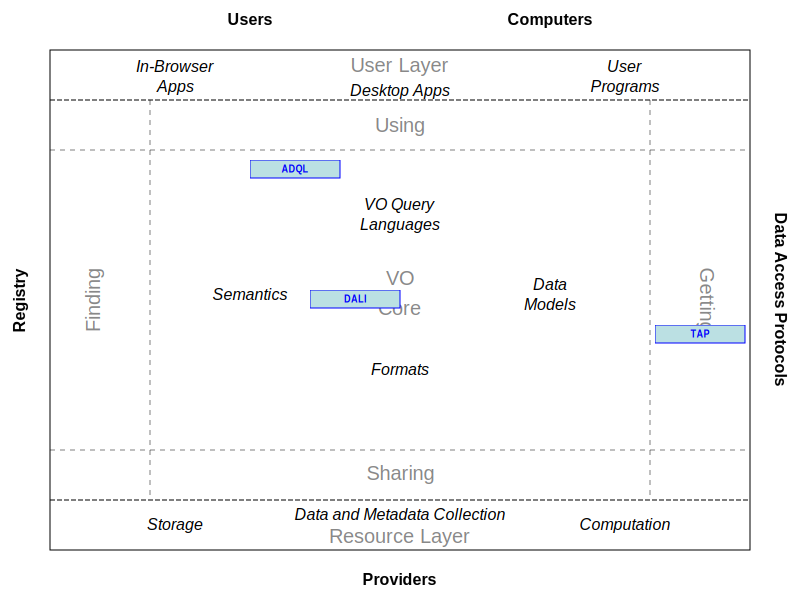
\includegraphics[width=0.9\textwidth]{archdiag.png}
\caption{Architecture diagram for this document}
\label{fig:archdiag}
\end{figure}

Fig.~\ref{fig:archdiag} shows the role this document plays within the
IVOA architecture \citep{note:VOARCH}.

\section{Astronomical Data Query Language (ADQL)}

This section describes the ADQL language specification. We will define in
subsequent sections the syntax for the special characters, reserved and non-
reserved words, identifiers and literals and then, finally, the syntax for
the query expression.

The formal notation for syntax of computing languages is often expressed
in the “Backus Naur Form” BNF. This syntax is used by popular tools for
producing parsers. Appendix A to this document provides the full BNF grammar
for ADQL. The following conventions are used through this document:

\begin{itemize}
    \item Optional items are enclosed in meta symbols \verb:[: and \verb:]:
    \item A group of items is enclosed in meta symbols \verb:{: and \verb:}:
    \item Repetitive item (zero or more times) are followed by \verb:...:
    \item Terminal symbols are enclosed by \verb:<: and \verb:>:
    \item Terminals of meta-symbol characters (\verb:=,[,],(,),<,>,*:) are surrounded by quotes (\verb:“:) to distinguish them from meta-symbols
    \item Case insensitiveness otherwise stated
\end{itemize}

\subsection{Characters, Keywords, Identifiers and Literals}
\subsubsection{Characters}

The language allows simple Latin letters (lower and upper case, i.e.
\verb:{aA-zZ}):, digits (\verb:{0-9}:) and the following special characters:

\begin{itemize}
\item space
\item single quote (\verb:’:)
\item double quote (\verb:“:)
\item percent (\verb:%:)
\item left and right parenthesis
\item asterisk (\verb:*:)
\item plus sign (\verb:+:)
\item minus sign (\verb:-:)
\item comma (\verb:,:)
\item period (\verb:.:)
\item solidus (\verb:/:)
\item colon (\verb.:.)
\item semicolon (\verb:;:)
\item less than operator (\verb:<:)
\item equals operator (\verb:=:)
\item greater than operator (\verb:>:)
\item underscore (\verb:_:)
\item ampersand (\verb:&:)
\item question mark (\verb:?:)
\item vertical bar (\verb:|:)
\end{itemize}

\subsubsection{Keywords and Identifiers}

Besides the character set, the language provides a list of reserved keywords
plus the syntax description for regular identifiers.

A reserved keyword has a special meaning in ADQL and cannot be used as
an identifier. These keywords must be enforced and should be extensive as
an escaping mechanism is already in place. We can extend the list of SQL92
reserved keywords to accommodate those useful for astronomical purposes and/or
present in a subset of vendor specific languages only (e.g. TOP). This leads
to the following list:

\begin{itemize}
    \item SQL reserved keywords:
\end{itemize}

\begin{verbatim}
ABSOLUTE, ACTION, ADD, ALL, ALLOCATE, ALTER, AND, ANY, ARE, AS, ASC,
ASSERTION, AT, AUTHORIZATION, AVG, BEGIN, BETWEEN, BIT, BIT_LENGTH,
BOTH, BY, CASCADE, CASCADED, CASE, CAST, CATALOG, CHAR, CHARACTER,
CHARACTER_LENGTH, CHAR_LENGTH, CHECK, CLOSE, COALESCE, COLLATE,
COLLATION, COLUMN, COMMIT, CONNECT, CONNECTION, CONSTRAINT,
CONSTRAINTS, CONTINUE, CONVERT, CORRESPONDING, COUNT, CREATE,
CROSS, CURRENT, CURRENT_DATE, CURRENT_TIME, CURRENT_TIMESTAMP,
CURRENT_USER, CURSOR, DATE, DAY, DEALLOCATE, DECIMAL, DECLARE,
DEFAULT, DEFERRABLE, DEFERRED, DELETE, DESC, DESCRIBE, DESCRIPTOR,
DIAGNOSTICS, DISCONNECT, DISTINCT, DOMAIN, DOUBLE, DROP, ELSE, END,
END-EXEC, ESCAPE, EXCEPT, EXCEPTION, EXEC, EXECUTE, EXISTS, EXTERNAL,
EXTRACT, FALSE, FETCH, FIRST, FLOAT, FOR, FOREIGN, FOUND, FROM,
FULL, GET, GLOBAL, GO, GOTO, GRANT, GROUP, HAVING, HOUR, IDENTITY,
IMMEDIATE, IN, INDICATOR, INITIALLY, INNER, INPUT, INSENSITIVE,
INSERT, INT, INTEGER, INTERSECT, INTERVAL, INTO, IS, ISOLATION,
JOIN, KEY, LANGUAGE, LAST, LEADING, LEFT, LEVEL, LIKE, LOCAL, LOWER,
MATCH, MAX, MIN, MINUTE, MODULE, MONTH, NAMES, NATIONAL, NATURAL,
NCHAR, NEXT, NO, NOT, NULL, NULLIF, NUMERIC, OCTET_LENGTH, OF, ON,
ONLY, OPEN, OPTION, OR, ORDER, OUTER, OUTPUT, OVERLAPS, PAD, PARTIAL,
POSITION, PRECISION, PREPARE, PRESERVE, PRIMARY, PRIOR, PRIVILEGES,
PROCEDURE, PUBLIC, READ, REAL, REFERENCES, RELATIVE, RESTRICT,
REVOKE, RIGHT, ROLLBACK, ROWS, SCHEMA, SCROLL, SECOND, SECTION,
SELECT, SESSION, SESSION_USER, SET, SIZE, SMALLINT, SOME, SPACE, SQL,
SQLCODE, SQLERROR, SQLSTATE, SUBSTRING, SUM, SYSTEM_USER, TABLE,
TEMPORARY, THEN, TIME, TIMESTAMP, TIMEZONE_HOUR, TIMEZONE_MINUTE,
TO, TRAILING, TRANSACTION, TRANSLATE, TRANSLATION, TRIM, TRUE,
UNION, UNIQUE, UNKNOWN, UPDATE, UPPER, USAGE, USER, USING, VALUE,
VALUES, VARCHAR, VARYING, VIEW, WHEN, WHENEVER, WHERE, WITH, WORK,
WRITE, YEAR, ZONE
\end{verbatim}

\begin{itemize}
    \item ADQL reserved keywords:
\end{itemize}

\begin{verbatim}
ABS, ACOS, ASIN, ATAN, ATAN2, CEILING, COS, DEGREES, EXP, FLOOR,
LOG, LOG10, MOD, PI, POWER, RADIANS, RAND, ROUND, SIN, SQRT, TAN,
TOP, TRUNCATE
\end{verbatim}

The identifiers are used to express, for example, a table or a column
reference name.

Both the identifiers and the keywords are case insensitive. They SHALL
begin with a letter \verb:{aA-zZ}:. Subsequent characters shall be letters,
underscores or digits \verb:{0-9}: as follows:

\begin{verbatim}
    <Latin_letter> [{ <underscore> | {<Latin_letter> | <digit>} }]
\end{verbatim}

For practical purposes the language specification should be able to address
reserved keyword and special character conflicts. To do so the language
provides a way to escape a non-compliant identifier by using the double
quote character as a delimiter.

ADQL allows making use of the same quoting mechanism to handle the case
sensitiveness if needed.

\subsubsection{Literals}

Finally we define the syntax rules for the different data types: string
and number.

A string literal is a character expression delimited by single quotes.

Literal numbers are expressed in BNF as follows:

\begin{verbatim}
    <unsigned_numeric_literal> ::=
        <exact_numeric_literal>
      | <approximate_numeric_literal>

    <exact_numeric_literal> ::=
        <unsigned_integer> [<period> [<unsigned_integer>]]
        | <period><unsigned_integer>

    <unsigned_integer> ::= <digit>...

    <approximate_numeric_literal> ::= <mantissa> E <exponent>

    <mantissa> ::= <exact_numeric_literal>

    <exponent> ::= <signed_integer>

    <signed_integer> ::= [<sign>] <unsigned_integer>

    <sign> ::= <plus_sign> | <minus_sign>
\end{verbatim}

Regarding the usage of other data types like datetime and timestamp, ADQL
can deal with them similarly to how SQL does: using the string literal
construct. As Relation Database Manager Systems (RDBMs) do, a service should
be able to implicitly convert strings to internal (datetime or timestamp)
form using a variety of techniques, where e.g. ISO 8601 is an acceptable
format. Therefore, as with other string representations, it should be up to
the service capability to understand such specific formats.

\subsection{Query syntax}

A full and complete syntax of the select statement can be found in “Appendix
A: BNF Grammar” at the \verb:<query_specification>: construct. Follows a simplified
syntax for the \verb:SELECT: statement showing the main constructs for the query
specification:

\begin{verbatim}
    SELECT
        [ ALL | DISTINCT ]
        [ TOP unsigned_integer ]
        {
             * |
             { value_expression [ [AS] column_name ] }, ...
         }
        FROM {
                {
                table_name [ [AS] identifier ] |
                ( SELECT ....) [ [AS] identifier ] |
                table_name [NATURAL]
                    [ INNER | { LEFT | RIGHT | FULL [OUTER] } ]
                    JOIN table_name
                    [ON search_condition | USING ( column_name,...) ]
                },
            ...
            }

        [ WHERE search_condition ]
        [ GROUP BY column_name, ... ]
        [ HAVING search_condition ]
        [ ORDER BY
            { column_name | unsigned_integer } [ ASC | DESC],
            ...
            ]
\end{verbatim}

The SELECT statement defines a query to some derived table(s) specified
in the FROM clause. As a result of this query, a subset of the table(s)
is returned. The order of the rows MAY be arbitrary unless ORDER BY clause
is specified. The order of the columns to return SHALL be the same as the
order specified in the selection list, or the order defined in the original
table if asterisk is specified. TOP n construct is used to return the first
n-rows. The selection list MAY include any numeric, string or geometry value
expression. In the following sections some constructs requiring further
description are presented.

\subsubsection{Table subqueries and Joins}

Table subqueries are present and can be used by some existing predicates
within the search condition (IN and BETWEEN most likely) or as an artifact
of building derived tables. Among the different types of join, ADQL supports
INNER and OUTER (LEFT, RIGHT and FULL) joins. If none is specified, the
default is INNER. All of these can be NATURAL or not. The join condition
does not support embedded sub joins.

\subsubsection{Search condition}

The search condition can be part of several other clauses: JOIN, HAVING and,
obviously, WHERE. Standard logical operators are present in its description
(AND, OR and NOT). Five different types of predicates are present in which
different types of reserved keywords or characters are used:

\begin{itemize}
    \item Standard comparison operators: \verb:=:, \verb:!=:, \verb:<>:, \verb:<:, \verb:>:, \verb:<=:, \verb:>=:
    \item \verb:BETWEEN:
    \item \verb:LIKE:
    \item \verb:NULL:
    \item \verb:EXISTS:
\end{itemize}

\subsection{Mathematical and Trigonometrical Functions}

ADQL declares a list of reserved keywords (section 2.1.2) which defines
a set of mathematical and trigonometrical function names. Their syntax,
usage and description are detailed in the following tables:

\begin{table}[thm]\footnotesize
    \begin{tabular}{|p{0.20\textwidth}|p{0.125\textwidth}|p{0.125\textwidth}|p{0.55\textwidth}|}
        \hline

        \hline
        \textbf{Name} &
        \textbf{Argument \newline data type} &
        \textbf{Return \newline data type} &
        \textbf{Description} \\

        \hline
        abs(x) &
        double&double &
        Returns the absolute value of x.\\

        \hline
        ceiling(x) &
        double&double &
        Returns the smallest double value that is not less than the argument x and is equal to a mathematical integer.\\

        \hline
        degrees(x) &
        double &
        double &
        Converts an angle to degrees. Argument x must be in radians.\\

        \hline
        exp(x) &
        double &
        double &
        Returns Euler’s number e raised to the power of x.\\

        \hline
        floor(x) &
        double &
        double &
        Returns the largest double value that is not greater than the argument x and is equal to a mathematical integer.\\

        \hline
        log(x) &
        double &
        double &
        Returns the natural logarithm (base e) of a double value. Value x must be greater than zero.\\
        
        \hline
        log10(x) &
        double &
        double &
        Returns the base 10 logarithm of a double value. Value x must be greater than zero.\\

        \hline
        mod(x, y) &
        double &
        double &
        Returns the remainder of y/x.\\
        
        \hline
        pi() &
        n/a &
        double &
        The \(\pi\) constant.\\
        
        \hline
        power(x, y) &
        x double \newline y double &
        double &
        Returns the value of the first argument raised to the power of the second argument.\\

        \hline
        radians(x) &
        double &
        double &
        Converts an angle to radians. Argument x must be in degrees.\\

        \hline
        sqrt(x) &
        double &
        double &
        Returns the positive square root of a double value.\\

        \hline
        rand(x) &
        integer &
        double &
        Returns a random value between 0.0 and 1.0, where x is a seed  value.\\

        \hline
        round(x, n) &
        x double \newline n integer &
        double &
        Rounds double value x to n number of decimal places, with the default being to round to the nearest integer.
        To round to the left of the decimal point, a negative number should be provided.\\

        \hline
        truncate(x, n) &
        x double \newline n integer &
        double &
        Returns the result of truncating the argument x to n decimal places.\\

        \hline
    \end{tabular}
    \caption{Mathematical functions}
    \label{table:extable}
\end{table}

\begin{table}[thm]\footnotesize
    \begin{tabular}{|p{0.20\textwidth}|p{0.125\textwidth}|p{0.125\textwidth}|p{0.55\textwidth}|}
        \hline

        \hline
        \textbf{Name} &
        \textbf{Argument \newline data type} &
        \textbf{Return \newline data type} &
        \textbf{Description} \\

        \hline
        acos(x) &
        double &
        double &
        Returns the arc cosine of an angle, in the range of 0 through \(\pi\) radians. Absolute value of x must be lower or equal than 1.0.\\

        \hline
        asin(x) &
        double &
        double &
        Returns the arc sine of an angle, in the range of -\(\pi\)/2 through \(\pi\)/2 radians. Absolute value of x must be and lower or equal than 1.0.\\

        \hline
        atan(x) &
        double &
        double &
        Returns the arc tangent of an angle, in the range of -\(\pi\)/2 through \(\pi\)/2 radians.\\
        
        \hline
        atan2(y,x) &
        double &
        double &
        Converts rectangular coordinates x,y to polar angle. It computes the arc tangent of y/x in the range of –\(\pi\) through \(\pi\) radians.\\

        \hline
        cos(x) &
        double &
        double &
        Returns the cosine of an angle, in the range of -1.0 through 1.0. Argument x must be in radians.\\

        \hline
        sin(x) &
        double &
        double &
        Returns the sine of an angle, in the range of -1.0 through 1.0. Argument x must be in radians.\\

        \hline
        tan(x) &
        double &
        double &
        Returns the tangent of an angle. Argument x must be in radians.\\

        \hline
    \end{tabular}
    \caption{Trigonometrical functions}
    \label{table:extable}
\end{table}

\subsection{Geometrical Functions}
\subsubsection{Overview}

In addition to the mathematical functions, ADQL provides a set of geometrical
functions to enhance the astronomical usage of the language. The list of
ADQL reserved keywords shown in Section 2.1.2 is therefore extended with
the following function names:

\begin{verbatim}
AREA, BOX, CENTROID, CIRCLE, CONTAINS, COORD1, COORD2,
COORDSYS, DISTANCE, INTERSECTS, POINT, POLYGON, REGION
\end{verbatim}

A special attention has to be paid to the REGION function. As can be seen more
in detail in Section 2.4.14, this construct is a general purpose function and
it takes a string value expression as argument. The format of the string is
to be specified by a service that accepts ADQL by referring to a standard
format. Currently STC/s (See [3] and [4]) is the only standardized string
representation a service can declare.

As can also be seen in the following sections, all these functions
have arguments being a geometrical, a string and/or a numerical value
expression. When these values represent spherical coordinates the units MUST
be in degrees (square degrees for area). If the cartesian coordinate system
is used, the vector coordinates MUST be normalized.

Regarding the legal ranges, for spherical coordinates, these SHOULD be [0, 360]
and [-90, 90]. In a cartesian coordinate system, there are no inherent limits
but the already mention constrain that vectors should be normalized. It remains
up to the service making use of ADQL to define the errors that should be raised
when using values outside these ranges.

For all these functions there is also a string parameter defining the
coordinate system. The allowed values MUST be defined by any service making
use of ADQL. A list of standard coordinate system literals can be found in
the appendix of the STC specification [3].

Generally speaking, all these geometrical functions cover three different
topics: data types, predicates and utility calculations. Each of these are
covered below.

%\subsubsubsection{Data Type Functions}

Certain functions represent geometry data types. These data types are BOX,
CENTROID, CIRCLE, POINT and POLYGON together with the generalized REGION data
type. The functions are similarly named and return a variable length binary
value. The semantics of these data types are based on the corresponding
concepts from the STC data model (See [3]).

Geometry data types are centered around the BNF construct
\verb:<value_expression>: which is central to data types within SQL.

\begin{verbatim}
    <value_expression> ::=
        <numeric_value_expression>
      | <string_value_expression>
      | <geometry_value_expression>
\end{verbatim}

A \verb:<geometry_value_expression>: does not simply cover data type functions
(POINT, CIRCLE etc) but must also allow for column values where a geometry
data type is stored in a column. Therefore, \verb:<geometry_value_expression>:
is expanded as

\begin{verbatim}
    <geometry_value_expression> ::= 
        <value_expression_primary>
      | <geometry_value_function>
\end{verbatim}

, where

\begin{verbatim}
    <geometry_value_function> ::=
        <box>
      | <centroid>
      | <circle>
      | <point>
      | <polygon>
      | <region>
\end{verbatim}

and \verb:<value_expression_primary>: makes possible to use a column reference.

%\subsubsubsection{Predicate Functions}

Functions CONTAINS and INTERSECTS each accept two geometry data types
and return 1 or 0 according to whether the relevant verb (e.g.: "contains") is
satisfied against the two input geometries; 1 represents true and 0 represents
false. Each of these functions can be assembled into a predicate:

\begin{verbatim}
    SELECT * FROM SDSS as s WHERE CONTAINS(POINT(...), CIRCLE(...)) = 1
\end{verbatim}

, where the ... would represent the constituent parts of a CIRCLE and POINT
geometry.

One would expect later additions to ADQL to add to this range of functions. For
example: equals, disjoint, touches, crosses, within, overlaps and relate
are possibilities.

%\subsubsubsection{Utility Functions}

Function COORDSYS extracts the coordinate system string from a given geometry. To do so it accepts a geometry expression and returns a calculated string value.

This function has been included as a string value function because it returns a simple string value. Hence

\begin{verbatim}
    <string_value_function> :: =
        <string_geometry_function> | <user_defined_function>

    <string_geometry_function> ::= <extract_coordsys>

    <extract_coordsys> ::=
        COORDSYS <left_paren> <geometry_value_expression> <right_paren>
\end{verbatim}

Other functions like AREA, COORD1, COORD2 and DISTANCE accept a geometry (or
two geometries in the case of DISTANCE) and return a calculated numeric value.

The Predicate and most of the Utility functions have been included as numeric
value functions because they return simple numeric values. Thus

\begin{verbatim}
    <numeric_value_function> ::=
        <trig_function>
      | <math_function>
      | <numeric_geometry_function>
      | <user_defined_function>
\end{verbatim}

, where

\begin{verbatim}
    <numeric_geometry_function> ::=
        <predicate_geometry_function>
      | <non_predicate_geometry_function>
\end{verbatim}


and

\begin{verbatim}
    <non_predicate_geometry_function> ::=
        AREA <left_paren> <geometry_value_expression> <right_paren>
      | COORD1 <left_paren> <coord_value> <right_paren>
      | COORD2 <left_paren> <coord_value> <right_paren>
      | DISTANCE <left_paren> <coord_value> <comma> <coord_value> <right_paren>
\end{verbatim}

and

\begin{verbatim}
    <predicate_geometry_function> ::= <contains> | <intersects>
\end{verbatim}

The following sections provide a detailed description for each geometrical
function. Its functionality and usage is described rather than going into
the BNF grammar details as above.

\subsubsection{AREA}

This function computes the area, in square degrees, of a given geometry.

For example, the area of a circle of one degree radius centered in a position
of (25.4, -20.0) degrees and defined according to the ICRS coordinate system
with GEOCENTER reference position would be written as follows:

\begin{verbatim}
    AREA(CIRCLE(‘ICRS GEOCENTER’, 25.4, -20.0, 1))
\end{verbatim}

The coordinates of the circle center could also be directly derived from
either a POINT function (See 2.4.12) or the coordinate’s column references:

\begin{verbatim}
    AREA(CIRCLE(‘ICRS GEOCENTER’, t.ra, t.dec, 1))
\end{verbatim}

, where \textit{t} would be the table and \textit{ra}, \textit{dec} the
column references for the circle centre.

Inappropriate geometries for this construct (e.g. POINT) SHOULD either return
zero or throw an error message, the later to be defined by the service making
use of ADQL.

\subsubsection{BOX}

This function expresses a box on the sky. A box is a special case of Polygon,
defined purely for convenience, and it corresponds semantically to the STC Box
region ([3], section 4.5.1.5). It is specified by a center position and size
(in both coordinates) defining a cross centered on the center position and
with arms extending, parallel to the coordinate axes at the center position,
for half the respective sizes on either side. The box’s sides are line
segments or great circles intersecting the arms of the cross in its end
points at right angles with the arms.

The function arguments specify the coordinate system, the center position
and both the width and height (arms) values, where

\begin{itemize}
    \item the coordinate system is a string value expression as defined in Section 2.4.1.
    \item the center position is a comma separated numeric duple, with units and legal ranges as defined in Section 2.4.1.
    \item and the arms are numeric value expressions in degrees.
\end{itemize}

For example, a function expressing a box of ten degrees centered in a position
(25.4, -20.0) in degrees and defined according to the ICRS coordinate system
with GEOCENTER reference position would be written as follows:

\begin{verbatim}
    BOX(‘ICRS GEOCENTER’, 25.4, -20.0, 10, 10)
\end{verbatim}

As another example, the coordinates of the center position could also be
extracted from either a POINT function (See 2.4.12) or the coordinate’s
column references:

\begin{verbatim}
    BOX(‘ICRS GEOCENTER’, t.ra, t.dec, 10, 10)
\end{verbatim}

, where \textit{t} would be the table and \textit{ra}, \textit{dec} the
column references for the center position.

To see what this function would return when listed in the select clause,
see Section 2.4.15.

\subsubsection{CENTROID}

This function computes the centroid of a given geometry and returns a POINT
(See 2.4.11).

For example, the centroid of a circle of one degree radius centered in a
position of (25.4, -20.0) degrees and defined according to the ICRS coordinate
system with GEOCENTER reference position would be written as follows :

\begin{verbatim}
    CENTROID(CIRCLE (‘ICRS GEOCENTER’, 25.4, -20.0, 1))
\end{verbatim}

\subsubsection{CIRCLE}

This function expresses a circular region on the sky (a cone in space) and
corresponds semantically to the STC Circle region ([3], section 4.5.1.2).. The
function arguments specify the coordinate system, the center position,
and the radius, where:

\begin{itemize}
    \item the coordinate system is a string value expression as defined in Section 2.4.1.
    \item the center position is a comma separated numeric duple, with units and legal ranges as defined in Section 2.4.1.
    \item and the radius is a numeric value expression in degrees.
\end{itemize}

For example, a function expressing a circle of one degree radius centered in a
position of (25.4, -20.0) degrees and defined according to the ICRS coordinate
system with GEOCENTER reference position, would be written as follows:

\begin{verbatim}
    CIRCLE(‘ICRS GEOCENTER’, 25.4, -20.0, 1)
\end{verbatim}

The coordinates of the center position could also be derived from either a
POINT function (See 2.4.12) or the coordinate’s column references:

\begin{verbatim}
    CIRCLE(‘ICRS GEOCENTER’, t.ra, t.dec, 1)
\end{verbatim}

, where \textit{t} would be the table and \textit{ra}, \textit{dec} the
column references for the center position.

To see what this function would return when listed in the select clause, see
Section 2.4.15.

\subsubsection{CONTAINS}

This numeric function determines if a geometry is wholly contained within
another. This is most commonly used to express the "point-in-shape" condition.

For example, to determine if a point with right ascension of 25 degrees
and declination of -19.5 degrees according to the ICRS coordinate system
with GEOCENTER reference position is within a circle of one degree radius
centered in a position of (25.4, -20.0) degrees and defined according to the
same coordinate system, we would make use of the CONTAINS function as follows:

\begin{verbatim}
    CONTAINS(
        POINT(‘ICRS GEOCENTER’, 25.0,-19.5),
        CIRCLE(‘ICRS GEOCENTER’, 25.4, -20.0, 1)
        )
\end{verbatim}

, where the CONTAINS function returns 1 (true) if the first argument is in
or on the boundary of the circle and 0 (false) otherwise. Thus, contains is
not symmetric in the meaning of the arguments. When used in the where clause
of a query, the value must be compared to 0 or 1 to form an SQL predicate:

\begin{verbatim}
    CONTAINS(
        POINT(‘ICRS GEOCENTER’, 25.0,-19.5),
        CIRCLE(‘ICRS GEOCENTER’, 25.4, -20.0, 1)
        ) = 1
\end{verbatim}

for "does contain" and

\begin{verbatim}
    CONTAINS(
        POINT(‘ICRS GEOCENTER’, 25.0,-19.5),
        CIRCLE(‘ICRS GEOCENTER’, 25.4, -20.0, 1)
        ) = 0
\end{verbatim}

for "does not contain".

The arguments to the CONTAINS function can be (literal) values created
from the geometry types or they can be single column names or aliases (for
geometry stored in a database table). Since the two argument geometries may
be expressed in different coordinate systems, the function is responsible
for converting one (or both). If it cannot do so, it SHOULD throw an error
message, to be defined by the service making use of ADQL.

\subsubsection{COORD1}

This function extracts the first coordinate value, in degrees, of a given
POINT (See 2.4.12) or column reference.

For example, the right ascension of a point with position (25, -19.5) in
degrees according to the ICRS coordinate system with GEOCENTER reference
position, would be obtained using the following expression:

\begin{verbatim}
    COORD1(POINT(‘ICRS GEOCENTER’, 25.0,-19.5))
\end{verbatim}

, being the result a numeric value of 25.0 degrees. The fist coordinate
could also be derived directly from a column reference as follows:

\begin{verbatim}
    COORD1(t.point)
\end{verbatim}
    
, where \textit{t} is the table and \textit{point} the column reference for
the POINT geometry stored in the database table.

\subsubsection{COORD2}

This function extracts the second coordinate value, in degrees, of a given
POINT (See 2.4.12) or column reference.

For example, the declination of a point with position (25, -19.5) in degrees
according to the ICRS coordinate system with GEOCENTER reference position,
would be obtained using the following expression:

\begin{verbatim}
    COORD2(POINT(‘ICRS GEOCENTER’, 25.0,-19.5))
\end{verbatim}

, being the result a numeric value of -19.5 degrees. The second coordinate
could also be derived directly from a column reference as follows:

\begin{verbatim}
    COORD2(t.point)
\end{verbatim}

, where \textit{t} is the table and \textit{point} the column reference for
the POINT geometry stored in the database table.

\subsubsection{COORDSYS}

This function extracts the coordinate system string value from a given
geometry.

As described in section 2.4.1, the allowed return values must be defined
by any service making use of ADQL, and a list of standard coordinate system
literals can be found in the STC specification [3].

For example, a function extracting the coordinate system of a point with
position (25, -19.5) in degrees according to the ICRS coordinate system with
GEOCENTER reference position, would be written as follows:

\begin{verbatim}
    COORDSYS(POINT(‘ICRS GEOCENTER’, 25.0,-19.5))
\end{verbatim}

, returning the ‘ICRS GEOCENTER’ string literal. As other samples above,
the coordinate system could also be derived from a column referencing any
other geometry data type:

\begin{verbatim}
    COORDSYS(t.circle)
\end{verbatim}

, where \textit{t} is the table and \textit{circle} the column reference
for the CIRCLE geometry stored in the database table.

\subsubsection{DISTANCE}

This function computes the arc length along a great circle between two points,
and returns a numeric value expression in degrees.

For example, a function computing the distance between two points of
coordinates (25,-19.5) and (25.4,-20) both expressed according to the
ICRS coordinate system with GEOCENTER reference position, would be written
as follows:

\begin{verbatim}
    DISTANCE(POINT(‘ICRS GEOCENTER’,25.0,-19.5),
    POINT(‘ICRS GEOCENTER’,25.4, -20.0))
\end{verbatim}

, where all numeric values and the returned arc-length are in degrees.

The distance between two points could also be derived from two columns
referencing POINT geometries stored in the database tables as follows:

\begin{verbatim}
    DISTANCE(t.p1,t.p2)
\end{verbatim}

, where \textit{t} would be the table and \textit{p1}, \textit{p2} the column
references for the POINT geometries.

Since the two argument points may be expressed in different coordinate systems,
the function is responsible for converting one (or both). If it cannot do
so, it SHOULD throw an error message, to be defined by the service making
use of ADQL.

\subsubsection{INTERSECTS}

This numeric function determines if two geometry values overlap. This is
most commonly used to express a "shape-vs-shape" intersection test.

For example, to determine whether a circle of one degree radius centered
in a position of (25.4, -20.0) degrees and defined according to the ICRS
coordinate system with GEOCENTER reference position overlaps with a box
of ten degrees centered in a position (20.0, -15.0) in degrees and defined
according to the same coordinate system, we would make use of the INTERSECTS
function as follows:

\begin{verbatim}
    INTERSECTS(
        CIRCLE(‘ICRS GEOCENTER’, 25.4, -20.0, 1),
        BOX(‘ICRS GEOCENTER’, 20.0, -15.0, 10, 10)
        )
\end{verbatim}

, where the INTERSECTS function returns 1 (true) if the two arguments overlap
and 0 (false) otherwise. When used in the where clause of a query, the value
must be compared to 0 or 1 to form an SQL predicate:

\begin{verbatim}
    INTERSECTS(CIRCLE(‘ICRS GEOCENTER’, 25.4, -20.0, 1),
    BOX(‘ICRS GEOCENTER’, 20.0, -15.0, 10, 10)
    ) = 1
\end{verbatim}

for "does intersect" and

\begin{verbatim}
    INTERSECTS(
        CIRCLE(‘ICRS GEOCENTER’, 25.4, -20.0, 1),
        BOX(‘ICRS GEOCENTER’, 20.0, -15.0, 10, 10)
        ) = 0
\end{verbatim}

for "does not intersect".

The arguments to the INTERSECTS function can be (literal) values created from
the geometry types or they can be single column names or aliases (for geometry
stored in a database table). Note that if one of the arguments is a POINT,
intersects is equivalent to contains (with the point argument first). Unlike
CONTAINS, the function’s arguments are commutative, e.g. INTERSECTS(a,
b) is equivalent to INTERSECTS(b, a). Since the two argument points may
be expressed in different coordinate systems, the function is responsible
for converting one (or both). If it cannot do so, it SHOULD throw an error
message, to be defined by the service making use of ADQL.

\subsubsection{POINT}

This function expresses a single location on the sky, and corresponds
semantically to an STC SpatialCoord ([3], section 4.4.2). The arguments
specify the coordinate system and the position, where:

\begin{itemize}
    \item the coordinate system is a string value expression as defined in Section 2.4.1.
    \item the position is a comma separated numeric duple, with units and legal ranges as defined in Section 2.4.1.
\end{itemize}

For example, a function expressing a point with right ascension of 25 degrees
and declination of -19.5 degrees according to the ICRS coordinate system
with GEOCENTER reference position, would be written as follows:

\begin{verbatim}
    POINT(‘ICRS GEOCENTER’, 25.0,-19.5)
\end{verbatim}

, where numeric values are in degrees. The coordinates of the POINT could
also be derived from the coordinate’s column references:

\begin{verbatim}
    POINT(‘ICRS GEOCENTER’, t.ra, t.dec)
\end{verbatim}
    
, where \textit{t} would be the table and \textit{ra}, \textit{dec} the
column references for the position.

The coordinates of a POINT could also be individually extracted using the
COORD1 and COORD2 functions (See 2.4.7 and 2.4.8).

To see what this function would return when listed in the select clause,
see Section 2.4.15.

\subsubsection{POLYGON}

This function expresses a region on the sky with sides denoted by great
circles passing through specified coordinates. It corresponds semantically
to the STC Polygon region ([3], section 4.5.1.4). The arguments specify the
coordinate system and three or more sets of 2-D coordinates, where:

\begin{itemize}
    \item the coordinate system is a string value expression as defined in Section 2.4.1.
    \item the coordinate sets are comma separated numeric duples, with units and legal ranges as defined in Section 2.4.1.
\end{itemize}

For example, a function expressing a triangle, whose vertices are (10.0,
-10.5), (20.0, 20.5) and (30.0,30.5) in degrees according to the ICRS
coordinate system with GEOCENTER reference position, would be written
as follows:

\begin{verbatim}
    POLYGON(‘ICRS GEOCENTER’, 10.0, -10.5, 20.0, 20.5, 30.0, 30.5)
\end{verbatim}
    
, where all numeric values are in degrees,

As for other geometries like BOX, CIRCLE and POINT, one could also derive
the coordinates from database column references instead:

\begin{verbatim}
    POLYGON(‘ICRS GEOCENTER’, t.ra, t.dec, 20.0, 20.5, 30.0, 30.5)
\end{verbatim}

, where t would be the table and ra, dec the column references for one of
the triangle’s corner position.

Thus, the polygon is a list of vertices in a single coordinate system, with
each vertex connected to the next along a great circle and the last vertex
implicitly connected to the first vertex.

\subsubsection{REGION}

This function provides a generic way of expressing a region represented by
a single string input parameter. The format of the string MUST be specified
by a service that accepts ADQL by referring to a standard format. Currently
STC/s is the only standardized string representation a service can declare.

For example, given a string serialization of an STC region, the REGION
function just embeds such literal within parenthesis in the following way:

\begin{verbatim}
    REGION(‘Convex ... Position ... Error ... Size’)
\end{verbatim}

A detailed description on how to use STC/s can be seen in the referenced
document [4]. Inappropriate geometries for this construct SHOULD throw an
error message, to be defined by the service making use of ADQL.

\subsubsection{Geometry in the SELECT clause}

Geometry values (literals or columns containing geometry values) may be
listed in the select clause, in which case they must be converted into a
text form. This text form will be identical to the way a literal value would
be specified in a query, including the geometry type (POINT, CIRCLE, BOX,
or POLYGON) and all arguments but excluding the required quotes around the
coordinate system string. For example, the query

\begin{verbatim}
    SELECT circle(‘ICRS GEOCENTER’, 1, 2, 0.5)
\end{verbatim}

could return

\begin{verbatim}
    CIRCLE(‘ICRS GEOCENTER ‘, 1.0, 2.0, 0.5)
\end{verbatim}

or equivalent. The case of the coordinate system string should be preserved;
the geometry type string is case insensitive. The output may alter the
numeric format by converting whole numbers to floating point (as in the
example above) but should not gratuitously add digits. Otherwise, numeric
output must conform to the rules for numeric expressions in the ADQL BNF.

\subsubsection{User Defined Functions}

ADQL also provides a placeholder to define user specific functions. Such
construct supports a variable list of parameters as input in the following way:

\begin{verbatim}
    <user_defined_function> ::=
        <user_defined_function_name> <left_paren>
            [
            <user_defined_function_param>
                [
                    {
                        <comma> <user_defined_function_param>
                    }...
                ]
            ]
        <right_paren>
\end{verbatim}

The function names can be qualified with a prefix to ease parsing of the
ADQL statement

\begin{verbatim}
    <user_defined_function_name> ::=
        [ <default_function_prefix> ] <regular_identifier>
\end{verbatim}

, while the function parameters are generic enough to support string,
numeric and geometrical expressions

\begin{verbatim}
    <user_defined_function_param> ::= <value_expression>
\end{verbatim}

If metadata on a user defined function is available, this should be used. For
example function names and cardinality of arguments should be checked against
metadata where available.

\appendix

\section{BNF Grammar}

An easier to navigate version of the BNF grammar can be found at \url{http://www.ivoa.net/internal/IVOA/IvoaVOQL/adql-bnf-v2.0.html}

\begin{verbatim}

    <ADQL_language_character> ::=
        <simple_Latin_letter>
      | <digit>
      | <SQL_special_character>

    <ADQL_reserved_word> ::=
        ABS
      | ACOS
      | AREA
      | ASIN
      | ATAN
      | ATAN2
      | BOX
      | CEILING
      | CENTROID
      | CIRCLE
      | CONTAINS
      | COORD1
      | COORD2
      | COORDSYS
      | COS
      | DEGREES
      | DISTANCE
      | EXP
      | FLOOR
      | INTERSECTS
      | LOG
      | LOG10
      | MOD
      | PI
      | POINT
      | POLYGON
      | POWER
      | RADIANS
      | REGION
      | RAND
      | ROUND
      | SIN
      | SQRT
      | TOP
      | TAN
      | TRUNCATE

    <SQL_embedded_language_character> ::=
        <left_bracket> | <right_bracket>

    <SQL_reserved_word> ::=
        ABSOLUTE | ACTION | ADD | ALL
      | ALLOCATE | ALTER | AND
      | ANY | ARE
      | AS | ASC
      | ASSERTION | AT
      | AUTHORIZATION | AVG
      | BEGIN | BETWEEN | BIT | BIT_LENGTH
      | BOTH | BY
      | CASCADE | CASCADED | CASE | CAST
      | CATALOG
      | CHAR | CHARACTER | CHAR_LENGTH
      | CHARACTER_LENGTH | CHECK | CLOSE | COALESCE
      | COLLATE | COLLATION
      | COLUMN | COMMIT
      | CONNECT
      | CONNECTION | CONSTRAINT
      | CONSTRAINTS | CONTINUE
      | CONVERT | CORRESPONDING | COUNT | CREATE | CROSS
      | CURRENT
      | CURRENT_DATE | CURRENT_TIME
      | CURRENT_TIMESTAMP | CURRENT_USER | CURSOR
      | DATE | DAY | DEALLOCATE
      | DECIMAL | DECLARE | DEFAULT | DEFERRABLE
      | DEFERRED | DELETE | DESC | DESCRIBE | DESCRIPTOR
      | DIAGNOSTICS
      | DISCONNECT | DISTINCT | DOMAIN | DOUBLE | DROP
      | ELSE | END | END-EXEC | ESCAPE
      | EXCEPT | EXCEPTION
      | EXEC | EXECUTE | EXISTS
      | EXTERNAL | EXTRACT
      | FALSE | FETCH | FIRST | FLOAT | FOR
      | FOREIGN | FOUND | FROM | FULL
      | GET | GLOBAL | GO | GOTO
      | GRANT | GROUP
      | HAVING | HOUR
      | IDENTITY | IMMEDIATE | IN | INDICATOR
      | INITIALLY | INNER | INPUT
      | INSENSITIVE | INSERT | INT | INTEGER | INTERSECT
      | INTERVAL | INTO | IS
      | ISOLATION
      | JOIN
      | KEY
      | LANGUAGE | LAST | LEADING | LEFT
      | LEVEL | LIKE | LOCAL | LOWER
      | MATCH | MAX | MIN | MINUTE | MODULE
      | MONTH
      | NAMES | NATIONAL | NATURAL | NCHAR | NEXT | NO
      | NOT | NULL
      | NULLIF | NUMERIC
      | OCTET_LENGTH | OF
      | ON | ONLY | OPEN | OPTION | OR
      | ORDER | OUTER
      | OUTPUT | OVERLAPS
      | PAD | PARTIAL | POSITION | PRECISION | PREPARE
      | PRESERVE | PRIMARY
      | PRIOR | PRIVILEGES | PROCEDURE | PUBLIC
      | READ | REAL | REFERENCES | RELATIVE | RESTRICT
      | REVOKE | RIGHT
      | ROLLBACK | ROWS
      | SCHEMA | SCROLL | SECOND | SECTION
      | SELECT
      | SESSION | SESSION_USER | SET
      | SIZE | SMALLINT | SOME | SPACE | SQL | SQLCODE
      | SQLERROR | SQLSTATE
      | SUBSTRING | SUM | SYSTEM_USER
      | TABLE | TEMPORARY
      | THEN | TIME | TIMESTAMP
      | TIMEZONE_HOUR | TIMEZONE_MINUTE
      | TO | TRAILING | TRANSACTION
      | TRANSLATE | TRANSLATION | TRIM | TRUE
      | UNION | UNIQUE | UNKNOWN | UPDATE | UPPER | USAGE
      | USER | USING
      | VALUE | VALUES | VARCHAR | VARYING | VIEW
      | WHEN | WHENEVER | WHERE | WITH | WORK | WRITE
      | YEAR
      | ZONE

    <SQL_special_character> ::=
        <space>
      | <double_quote>
      | <percent>
      | <ampersand>
      | <quote>
      | <left_paren>
      | <right_paren>
      | <asterisk>
      | <plus_sign>
      | <comma>
      | <minus_sign>
      | <period>
      | <solidus>
      | <colon>
      | <semicolon>
      | <less_than_operator>
      | <equals_operator>
      | <greater_than_operator>
      | <question_mark>
      | <underscore>
      | <vertical_bar>

    <ampersand> ::= &

    <approximate_numeric_literal> ::= <mantissa>E<exponent>

    <area> ::= AREA <left_paren> <geometry_value_expression> <right_paren>

    <as_clause> ::= [ AS ] <column_name>

    <asterisk> ::= *

    <between_predicate> ::=
        <value_expression> [ NOT ] BETWEEN
        <value_expression> AND <value_expression>

    <boolean_factor> ::= [ NOT ] <boolean_primary>

    <boolean_primary> ::=
      | <left_paren> <search_condition> <right_paren>
        <predicate>
ZRQ

    <boolean_term> ::=
        <boolean_factor>
      | <boolean_term> AND <boolean_factor>

    <box> ::=
        BOX <left_paren>
            <coord_sys>
            <comma> <coordinates>
            <comma> <numeric_value_expression>
            <comma> <numeric_value_expression>
        <right_paren>

    <catalog_name> ::= <identifier>

    <centroid> ::=
        CENTROID <left_paren>
            <geometry_value_expression>
        <right_paren>

    <character_factor> ::= <character_primary>

    <character_primary> ::=
        <value_expression_primary>
      | <string_value_function>

    <character_representation> ::= <nonquote_character> | <quote_symbol>

    <character_string_literal> ::=
        <quote> [ <character_representation>... ] <quote>
        [
            {
                <separator>...
                <quote> [ <character_representation>... ] <quote>
            }...
        ]

    <character_value_expression> ::= <concatenation> | <character_factor>

    <circle> ::=
        CIRCLE <left_paren>
            <coord_sys>
            <comma> <coordinates>
            <comma> <radius>
        <right_paren>

    <colon> ::= :

    <column_name> ::= <identifier>

    <column_name_list> ::= <column_name> [ { <comma> <column_name> }... ]

    <column_reference> ::= [ <qualifier> <period> ] <column_name>

    <comma> ::= ,

    <comment> ::= <comment_introducer> [ <comment_character>... ] <newline>

    <comment_character> ::= <nonquote_character> | <quote>

    <comment_introducer> ::= <minus_sign><minus_sign> [<minus_sign>...]

    <comp_op> ::=
        <equals_operator>
      | <not_equals_operator>
      | <less_than_operator>
      | <greater_than_operator>
      | <less_than_or_equals_operator>
      | <greater_than_or_equals_operator>

    <comparison_predicate> ::=
        <value_expression> <comp_op> <value_expression>

    <concatenation> ::=
        <character_value_expression>
        <concatenation_operator>
        <character_factor>

    <concatenation_operator> ::= ||

    <contains> ::=
        CONTAINS <left_paren>
            <geometry_value_expression> <comma> <geometry_value_expression>
        <right_paren>

    <coord1> ::= COORD1 <left_paren> <coord_value> <right_paren>

    <coord2> ::= COORD2 <left_paren> <coord_value> <right_paren>

    <coord_sys> ::= <string_value_expression>

    <coord_value> ::= <point> | <column_reference>

    <coordinate1> ::= <numeric_value_expression>

    <coordinate2> ::= <numeric_value_expression>

    <coordinates> ::= <coordinate1> <comma> <coordinate2>

    <correlation_name> ::= <identifier>

    <correlation_specification> ::= [ AS ] <correlation_name>

    <default_function_prefix> ::=
ZRQ

    <delimited_identifier> ::=
        <double_quote> <delimited_identifier_body> <double_quote>

    <delimited_identifier_body> ::= <delimited_identifier_part>...

    <delimited_identifier_part> ::=
        <nondoublequote_character> | <double_quote_symbol>

    <delimiter_token> ::=
        <character_string_literal>
        | <delimited_identifier>
        | <SQL_special_character>
        | <not_equals_operator>
        | <greater_than_or_equals_operator>
        | <less_than_or_equals_operator>
        | <concatenation_operator>
        | <double_period>
        | <left_bracket>
        | <right_bracket>

    <derived_column> ::= <value_expression> [ <as_clause> ]

    <derived_table> ::= <table_subquery>

    <digit> ::= 0 | 1 | 2 | 3 | 4 | 5 | 6 | 7 | 8 | 9

    <distance_function> ::=
        DISTANCE <left_paren>
            <coord_value> <comma> <coord_value>
        <right_paren>

    <double_period> ::= ..

    <double_quote> ::= "

    <double_quote_symbol> ::= <double_quote><double_quote>

    <equals_operator> ::= =

    <exact_numeric_literal> ::=
        <unsigned_integer> [ <period> [ <unsigned_integer> ] ]
      | <period> <unsigned_integer>

    <exists_predicate> ::= EXISTS <table_subquery>

    <exponent> ::= <signed_integer>

    <extract_coordsys> ::=
        COORDSYS <left_paren>
            <geometry_value_expression>
        <right_paren>

    <factor> ::= [ <sign> ] <numeric_primary>

    <from_clause> ::=
        FROM <table_reference>
	    [ { <comma> <table_reference> }... ]

    <general_literal> ::= <character_string_literal>

    <general_set_function> ::=
        <set_function_type> <left_paren>
            [ <set_quantifier> ] <value_expression>
        <right_paren>

    <geometry_value_expression> ::=
        <value_expression_primary > | <geometry_value_function>

    <geometry_value_function> ::=
        <box>
      | <centroid>
      | <circle>
      | <point>
      | <polygon>
      | <region>

    <greater_than_operator> ::= >

    <greater_than_or_equals_operator> ::= >=

    <group_by_clause> ::= GROUP BY <grouping_column_reference_list>

    <grouping_column_reference> ::= <column_reference>

    <grouping_column_reference_list> ::=
        <grouping_column_reference>
        [ { <comma> <grouping_column_reference> }... ]

    <having_clause> ::= HAVING <search_condition>

    <identifier> ::= <regular_identifier> | <delimited_identifier>

    <in_predicate> ::=
        <value_expression> [ NOT ] IN <in_predicate_value>

    <in_predicate_value> ::=
        <table_subquery> | <left_paren> <in_value_list> <right_paren>

    <in_value_list> ::=
        <value_expression> { <comma> <value_expression> } ...

    <intersects > ::=
        INTERSECTS <left_paren>
            <geometry_value_expression> <comma> <geometry_value_expression>
        <right_paren>

    <join_column_list> ::= <column_name_list>

    <join_condition> ::= ON <search_condition>

    <join_specification> ::= <join_condition> | <named_columns_join>

    <join_type> ::=
        INNER | <outer_join_type> [ OUTER ]

    <joined_table> ::=
        <qualified_join> | <left_paren> <joined_table> <right_paren>

    <keyword> ::= <SQL_reserved_word> | <ADQL_reserved_word>

    <left_bracket> ::= [

    <left_paren> ::= (

    <less_than_operator> ::= <

    <less_than_or_equals_operator> ::= <=

    <like_predicate> ::=
        <match_value> [ NOT ] LIKE <pattern>

    <mantissa> ::= <exact_numeric_literal>

    <match_value> ::= <character_value_expression>

    <math_function> ::=
        ABS <left_paren> <numeric_value_expression> <right_paren>
      | CEILING <left_paren> <numeric_value_expression> <right_paren>
      | DEGREES <left_paren> <numeric_value_expression> <right_paren>
      | EXP <left_paren> <numeric_value_expression> <right_paren>
      | FLOOR <left_paren> <numeric_value_expression> <right_paren>
      | LOG <left_paren> <numeric_value_expression> <right_paren>
      | LOG10 <left_paren> <numeric_value_expression> <right_paren>
      | MOD <left_paren>
            <numeric_value_expression> <comma> <numeric_value_expression>
        <right_paren>
      | PI <left_paren><right_paren>
      | POWER <left_paren>
            <numeric_value_expression> <comma> <numeric_value_expression> >
ZRQ
        <right_paren>
      | RADIANS <left_paren> <numeric_value_expression> <right_paren>
      | RAND <left_paren> [ <unsigned_integer> ] <right_paren>
      | ROUND <left_paren>
            <numeric_value_expression> [ <comma> <signed_integer>]
        <right_paren>
      | SQRT <left_paren> <numeric_value_expression> <right_paren>
      | TRUNCATE <left_paren>
            <numeric_value_expression>
            [ <comma> <signed_integer>]
        <right_paren>

    <minus_sign> ::= -

    <named_columns_join> ::=
        USING <left_paren>
            <join_column_list>
        <right_paren>

    <newline> ::=

    <non_predicate_geometry_function> ::=
        <area>
      | <coord1>
      | <coord2>
      | <distance>

    <nondelimiter_token> ::=
        <regular_identifier>
      | <keyword>
      | <unsigned_numeric_literal>

    <nondoublequote_character> ::=
ZRQ

    <nonquote_character> ::=
ZRQ

    <not_equals_operator> ::= <not_equals_operator1> | <not_equals_operator2>

    <not_equals_operator1> ::= <>

    <not_equals_operator2> ::= !=

    <null_predicate> ::= <column_reference> IS [ NOT ] NULL

    <numeric_geometry_function> ::=
        <predicate_geometry_function> | <non_predicate_geometry_function>

    <numeric_primary> ::=
        <value_expression_primary>
      | <numeric_value_function>

    <numeric_value_expression> ::=
        <term>
      | <numeric_value_expression> <plus_sign> <term>
      | <numeric_value_expression> <minus_sign> <term>

    <numeric_value_function> ::=
        <trig_function>
      | <math_function>
      | <numeric_geometry_function >
      | <user_defined_function>

    <order_by_clause> ::= ORDER BY <sort_specification_list>

    <ordering_specification> ::= ASC | DESC

    <outer_join_type> ::= LEFT | RIGHT | FULL

    <pattern> ::= <character_value_expression>

    <percent> ::= %

    <period> ::= .

    <plus_sign> ::= +

    <point> ::=
        POINT <left_paren>
            <coord_sys> <comma> <coordinates>
        <right_paren>

    <polygon> ::=
        POLYGON <left_paren>
            <coord_sys>
            <comma> <coordinates>
            <comma> <coordinates>
            { <comma> <coordinates> } ?
        <right_paren>

    <predicate> ::=
        <comparison_predicate>
      | <between_predicate>
      | <in_predicate>
      | <like_predicate>
      | <null_predicate>
      | <exists_predicate>

    <predicate_geometry_function> ::= <contains> | <intersects>

    <qualified_join> ::=
        <table_reference> [ NATURAL ] [ <join_type> ] JOIN
        <table_reference> [ <join_specification> ]

    <qualifier> ::= <table_name> | <correlation_name>

    <query_expression> ::=
        <query_specification>
      | <joined_table>

    <query_specification> ::=
        SELECT
            [ <set_quantifier> ]
            [ <set_limit> ]
            <select_list>
            <table_expression>

    <question_mark> ::= ?

    <quote> ::= '

    <quote_symbol> ::= <quote> <quote>

    <radius> ::= <numeric_value_expression>

    <region> ::=
        REGION <left_paren> <string_value_expression> <right_paren>

    <regular_identifier> ::=
        <simple_Latin_letter>...
        [ { <digit> | <simple_Latin_letter> | <underscore> }... ]

    <right_bracket> ::= ]

    <right_paren> ::= )

    <schema_name> ::= [ <catalog_name> <period> ] <unqualified_schema name>

    <search_condition> ::=
        <boolean_term>
      | <search_condition> OR <boolean_term>

    <select_list> ::=
        <asterisk>
      | <select_sublist> [ { <comma> <select_sublist> }... ]

    <select_sublist> ::= <derived_column> | <qualifier> <period> <asterisk>

    <semicolon> ::= ;

    <separator> ::= { <comment> | <space> | <newline> }...

    <set_function_specification> ::=
        COUNT <left_paren> <asterisk> <right_paren>
      | <general_set_function>
ZRQ

    <set_function_type> ::= AVG | MAX | MIN | SUM | COUNT

    <set_limit> ::= TOP <unsigned_integer>

    <set_quantifier> ::= DISTINCT | ALL

    <sign> ::= <plus_sign> | <minus_sign>

    <signed_integer> ::= [ <sign> ] <unsigned_integer>

    <simple_Latin_letter> ::=
        <simple_Latin_upper_case_letter>
      | <simple_Latin_lower_case_letter>

    <simple_Latin_lower_case_letter> ::=
        a|b|c|d|e|f|g|h|i|j|k|l|m|n|o|p|q|r|s|t|u|v|w|x|y|z

    <simple_Latin_upper_case_letter> ::=
        A|B|C|D|E|F|G|H|I|J|K|L|M|N|O|P|Q|R|S|T|U|V|W|X|Y|Z

    <solidus> ::= /

    <sort_key> ::= <column_name> | <unsigned_integer>

    <sort_specification> ::=
        <sort_key> [ <ordering_specification> ]

    <sort_specification_list> ::=
        <sort_specification> [ { <comma> <sort_specification> }... ]

    <space> ::=

    <string_geometry_function> ::= <extract_coordsys>

    <string_value_expression> ::= <character_value_expression>

    <string_value_function> ::=
        <string_geometry_function> | <user_defined_function>

    <subquery> ::= <left_paren> <query_expression> <right_paren>

    <table_expression> ::=
        <from_clause>
        [ <where_clause> ]
        [ <group_by_clause> ]
        [ <having_clause> ]
        [ <order_by_clause> ]

    <table_name> ::= [ <schema_name> <period> ] <identifier>

    <table_reference> ::=
        <table_name> [ <correlation_specification> ]
      | <derived_table> <correlation_specification>
      | <joined_table>

    <table_subquery> ::= <subquery>

    <term> ::=
        <factor>
      | <term> <asterisk> <factor>
      | <term> <solidus> <factor>

    <token> ::=
        <nondelimiter_token> | <delimiter_token>

    <trig_function> ::=
        ACOS <left_paren> <numeric_value_expression> <right_paren>
      | ASIN <left_paren> <numeric_value_expression> <right_paren>
      | ATAN <left_paren> <numeric_value_expression> <right_paren>
      | ATAN2 <left_paren>
            <numeric_value_expression> <comma> <numeric_value_expression>
        <right_paren>
      | COS <left_paren> <numeric_value_expression> <right_paren>
      | COT <left_paren> <numeric_value_expression> <right_paren>
      | SIN <left_paren> <numeric_value_expression> <right_paren>
      | TAN <left_paren> <numeric_value_expression> <right_paren>

    <underscore> ::= _

    <unqualified_schema name> ::= <identifier>

    <unsigned_integer> ::= <digit>...

    <unsigned_literal> ::= <unsigned_numeric_literal> | <general_literal>

    <unsigned_numeric_literal> ::=
        <exact_numeric_literal> | <approximate_numeric_literal>

    <unsigned_value_specification> ::= <unsigned_literal>

    <user_defined_function> ::=
        <user_defined_function_name> <left_paren>
                [
                    <user_defined_function_param>
                [
                    {
                        <comma> <user_defined_function_param>
                    }...
                ]
                ]
            <right_paren>

    <user_defined_function_name> ::=
        [ <default_function_prefix> ] <regular_identifier>

    <user_defined_function_param> ::= <value_expression>

    <value_expression> ::=
        <numeric_value_expression>
      | <string_value_expression>
      | <geometry_value_expression>

    <value_expression_primary> ::=
        <unsigned_value_specification>
        | <column_reference>
        | <set_function_specification>
        | <left_paren> <value_expression> <right_paren>

    <vertical_bar> ::= |

    <where_clause> ::= WHERE <search_condition>

\end{verbatim}

\section{Changes from Previous Versions}

\subsection{Changes from ADQL-2.0}




\bibliography{ivoatex/ivoabib}

\end{document}

